% This example is a LaTeX document showing how to use the lmproj class to
% write your report. The chapter headings are by no means prescriptive. Instead
% use an appropriate report structure for your project as you see fit.
% Use pdflatex and bibtex to process the file, creating a PDF file as output 
% (there is no need to use dvips when using pdflatex).

% Modified 

\documentclass{lmproj}
\usepackage{amsmath}
\usepackage{listings}
\usepackage{amssymb}
\usepackage{subfigure}
\usepackage{graphicx}
\begin{document}
\title{Large-Scale Learning: Query-driven Machine Learning over Distributed Data}
\author{Kurt Portelli \\
        Natascha Harth \\
        Ruben Giaquinta \\
        Xu Zhang \\
        Monica Gandhi}
\date{18 December 2015}
\maketitle
\begin{abstract}
We study a novel solution to executing aggregation queries more specifically AVERAGE queries over large scale-data. We investigate cases where the owners restrict data access such that only aggregation operators can be used. It can also be extended to scenarios where access to the data is limited due to cost or slowness. Using distance-based queries with aggregation operators we are able to gain insight on how to best cluster the underlying data. The useful information are the results derived from the aggregation queries which are then clustered based on the distance based queries allowing us to predict the results of new and unseen queries. We study this approach which is called query-driven machine learning and evaluate its performance.

\end{abstract}
\educationalconsent
\tableofcontents
%==============================================================================
\chapter{Introduction}
\label{intro}
With the enormous improvements in performance and price in both data storage devices and network infrastructure it is now very cheap to store data. Since such large amounts of data is now accessible this has created a need and opportunity for machine learning algorithms.\cite{LargeScaleOnlineLearning} The challenge nowadays is not to store large amounts of data but to make it as accessible as possible. It is very difficult to query these datasets and return results interactively. According to L.Bottou and Y.Le Cunn\cite{LargeScaleOnlineLearning} these technological improvements have outran the exponential evolution of computing power. Thus, we must rely more on learning algorithms to process these large amounts of data with comparatively less computing power. These algorithms are typically split into online and batch. Online algorithms quickly process large datasets by adjusting their parameters as fresh data is inputted. On the other hand batch algorithms keep iterating over the dataset to achieve the optimum solution. It is then argued that online outperform batch algorithms due to the fact they do not iterate over a dataset.\cite{LargeScaleOnlineLearning}

In this work we are going to assume we are dealing with datasets which we don't have access to, or data access is too costly. In a real world scenario this can occur for a variety of reasons. It might be that the dataset is just too large to go through it, or the third party REST API service that is being used has a cost for each query that is made. Another requirement might be that this third party company does not allow a copy of their data to be held. Thus, batch algorithms won't be able to iterate through the whole dataset or it might be too costly to do so example in a Cloud setting. 

We will be investigating the use of online clustering in machine learning with the aim to finally be able to predict the results of queries without running them on the dataset. We will also be using a query driven approach \cite{LearningDNN} which will allow us to only quantize the important areas inside the data space. This approach creates various subspaces of interest  which are determined by a focal point in space and radius. The AVERAGE aggregation operator will be studied to gain an insight on how best to cluster the underlying dataset. The goal is to use the results of the queries issued to cluster the underlying data. Online clustering is used because these results represent a stream of infinite data which the clustering can learn over time.

Before going in detail about the training set generation, learning and prediction process, in the following section traditional algorithms and related work are going to be discussed to better compare our achievements.

%==============================================================================
\chapter{Related work}
\label{relatedWork}
The general approach in learning a large multi-dimensional dataset is to investigate the dataset as a whole and estimate the probability density function. G.Cormode et al. in \cite{Synopses} describes the well established techniques used in aggregate query processing. They mention histograms, self tuning histograms, sketches, sampling and wavelets. As C.Anagnostopoulos and P.Triantafillou argue in \cite{learningCount} these techniques assume that they have access to the actual data set, thus can store and preserve the statistical model created. For example to be kept up to date, histograms need to scan all the data. On the other hand Self-tuning histograms execute additional queries to adjust the statistical model accordingly.

GENHIST\cite{Genhist} is one of the variations of histograms with the same target, to find an approximate density function using a grid. GENHIST achieves this by iteratively split the dataset into regular grids and find the dense areas. In each iteration the density of each bucket with the surrounding buckets is smoothed. The innovation behind this is that in each iteration buckets may overlap thus, revealing new information and a more accurate density function. In each iteration buckets are removed which effect the number of iterations, for example a high value can result in losing important detail. Although the number of iterations is a constant number which depends on the parameters given this still scales directly with the size of the dataset. Each iteration involves doing one pass over the data and since the number of iterations is constant, the running time of the algorithm is constant.\cite{Genhist}

As the dataset changes over time the GENHIST algorithm has to be run again to update the probability density function. As the dataset increases in size, traditional histograms such as GENHIST fail to scale well due to the fact that they regularly need to be rebuilt to update the statistical model creating a substantial overhead. It is then noted that the statistical models created by histograms only consider the data distribution without taking into consideration the query pattern of users.\cite{learningCount} Thus, this is not suitable for what we want to achieve, as we are interested in a constructing a model that relies on the query distribution and data distribution. Self-tuning histograms (STH) were proposed to address this by using the cardinality of a query's result to adjust the statistical model. STH still have a fundamental limitation which is the necessity of reading all the dataset because it needs to calculate the probability density function. The use of wavelets, sketches and sampling are also discussed in \cite{learningCount} with the conclusion that they are not viable since they need to access the raw data to create and maintain their structures.

In \cite{learningCount} the query driven approach is discussed in detail and compared to the techniques mentioned above. The query driven approach is very useful in the scenario where one does not have access to the data or it is very costly to access the data (maybe due to size, cost, location). The idea behind this approach is that a training set containing a list of queries with their corresponding output is given. After learning this training set the algorithm should be able to predict the output without running the query. Although the training set is extracted from the dataset it is independent from the size of the dataset. Thus the size of the dataset will not impact the performance and the quality of the prediction fully depends on the training set and prediction algorithm used.

C.Anagnostopoulos and P.Triantafillou\cite{learningCount} discuss how this training set can be manipulated to allow the algorithm to predict results from queries as fast and accurate as possible. It is accepted that new queries might not be found in the training set thus a way to identify how close a query is to another is to use euclidean distance. One can go through all the training set, find the closest training query and then return the result of that query. This solution would increase linearly on the size of the training set. But, some queries might be redundant since they are very close to other existing queries while others might be significantly more important since they define another whole separate user interest. This shows the importance to extract information from the query space and be able to find the interest areas. Thus, the solution would be to cluster similar queries into a smaller set of representative queries notated by \textit{L}.

To arrive at the prediction stage each representative query is assigned a representative result. The representative results are continuously updated while learning and moved around the data space depending on the training set. If the training space is large enough the representative queries and results should converge to represent what is actually inside the raw data. The clear advantage is that the size of \textit{L} is smaller than the size of the training set which in turn is smaller than the raw data.\cite{learningCount}

Learning can easily be stopped and continued without the need to start from scratch. This approach makes prediction very fast since each new query is associated with a closest representative query and the representative result given. In case the actual result is known the prediction error can be calculated by checking the difference between the actual and predicted result.\cite{learningCount}

%==============================================================================
\chapter{Machine Learning Clustering Algorithms}
\label{clustering}

\section{Large Data Set Clustering}
Dealing with huge data spaces is not a simple issue. In order to do that, sometimes it is necessary either to reduce the scale of the problem or search for patterned distributions of objects within the data space. The latter feature can be useful to analyze and distinguish between possible areas of interest and less populated partitions of the space. To achieve this in machine learning, clustering techniques are commonly used. The problem of cluster analysis consists in grouping a set of objects, the data set, in clusters (groups), according to similar features. Similarity among objects is mainly related to the concept of Euclidean distance. In this section some clustering algorithms will be presented.

\subsection{Nearest Neighbour - Average Data}
\subsubsection{The Algorithm}
The Nearest Neighbour algorithm is one of the simplest methods for classification. The algorithm, given a finite set of d-dimensional vectors $X=\{x^t\}_{t=1}^{N}$, each with a class label, and a defined constant $k$, partitions the space classifying each point $x \in X$ as the majority class between the $k$ nearest neighbors. In order to find the $k$ nearest neighbors, the function calculates for each $x \in X$ the Euclidean distance between $x$ and $x'$, $\forall x' \in X$.

\subsubsection{Implementation}
The method classify, implemented within the class \textit{Tools} for Online K-Means, can be seen as a frame of the particular case of the Nearest Neighbour algorithm with $k=1$. The function computes the Euclidean distance between a point and all the centroids calling the \textit{distance} method; the index of the nearest centroid is returned in order to assign the point to its cluster.
\lstinputlisting[language=Java, basicstyle=\tiny, firstline=11,lastline=31]{ToolsKM.java}

\subsection{Offline K-Means}
\subsubsection{The Algorithm}
Batch K-Means\cite{Clustering} is the oldest and most simple clustering method; it is however very efficient. The algorithm, given a finite data set of d-dimensional vectors $X=\{x^t\}_{t=1}^{N}$ and $k$ \textit{centroids}, or \textit{codebook vectors}, $m_j,j=1,...,k$, partitions the data set into $k$ clusters in order to minimize the so called total \textit{reconstruction error}, defined as follows:
\begin{equation}
E(\{m_i\}^k_{i=1}|X)=\underset{t}{\sum}\underset{i}{\sum}b_i^t
\end{equation}
where
\begin{equation}
b_i^t=
\begin{cases}
1 & if \parallel x^t -m_i \parallel = min_j \parallel x^t - m_j \parallel \\
0 & otherwise.
\end{cases}
\end{equation}
Therefore, $x^t$ is represented by $m_i$ with an error proportional to the Euclidean distance $\parallel x^t - m_j \parallel$. The procedure starts initializing $m_i$ randomly; at each iteration $b_i^t$ is calculated for all $x^t$ and $m_i$ is updated according to the following rule:
\begin{equation}
m_i=\dfrac{\sum_t b_i^t x^t}{\sum_t b_i^t}.
\end{equation}
The algorithm terminates if any of the \textit{codebook vectors} $m_i$ hasn't been changed during the update step. Upon termination the function returns the \textit{codebook verctors}.

\subsubsection{Implementation}
The Batch K-Means was implemented in Java. The Cluster class has two objects, an \textit{ArrayList} of \textit{points} representing all the points belonging to the cluster, and a \textit{centroid}, the \textit{codebook vector}.
Centroids are initialized, inside the constructor, with randomly chosen points from the data set.
\lstinputlisting[language=Java, basicstyle=\tiny, firstline=33,lastline=46]{OfflineKmeansN.java}
The update function searches for the nearest \textit{codebook vector}.
\lstinputlisting[language=Java, basicstyle=\tiny, firstline=53,lastline=79]{OfflineKmeansN.java}
At a later stage the method applies the update rule for each of the \textit{codebook vectors}, counting the number of updated \textit{centroids}. A centroid will not be updated if the coordinates need to be shifted of a value under the default convergence error $0.05$.
\lstinputlisting[language=Java, basicstyle=\tiny, firstline=81,lastline=139]{OfflineKmeansN.java}
The function terminates if the value of the variable counting the number of modified centroids is equal to the number of clusters $counter == Clusters.size()$.

\begin{figure}[ht]
	\centering
	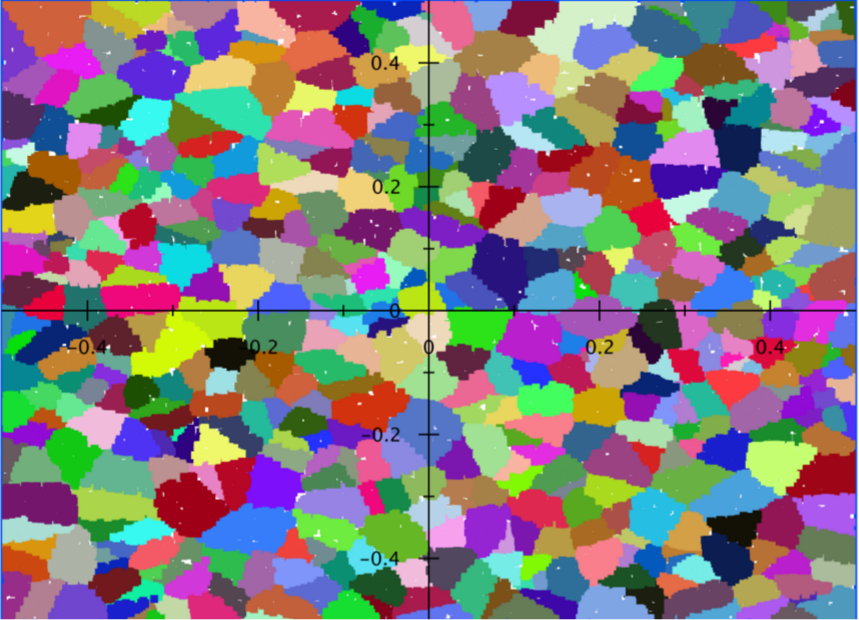
\includegraphics[width=0.6\linewidth]{batchkm.png}
   \caption[BatchKM]{Batch K-Means on a huge dataset with k=500.}
\end{figure}


\subsection{Online K-Means}
\subsubsection{The Algorithm}
The Batch K-Means cannot, or at least not efficiently, deal with huge data sets. Storing a vast amount of data in internal memory can be a serious issue. In order to avoid this problem, Online K-Means\cite{Clustering} does not store input data. Therefore, the algorithm initialize $k$ random \textit{codebook vectors} $m_j,j=1,...,k$ from the training set $X$. For all $x^t \in X$, randomly chosen, the update function computes:  
\begin{equation}
i \longleftarrow arg min_j \parallel x^t - m_j \parallel
\end{equation}
\begin{equation}
m_i \longleftarrow m_i + \eta (x^t - m_i)
\end{equation}
until $m_i$ converge. The constant $\eta$ is called the learning rate. Keeping $\eta$ large enhance accuracy but makes $m_i$ oscillate; therefore, for a matter of convergence $\eta$ need to be set around zero, losing accuracy.

\subsubsection{Implementation}
The Online K-means was implemented in Java as well. The update method is presented below:
\lstinputlisting[language=Java, basicstyle=\tiny, firstline=23,lastline=40]{OnlineKmeans.java}
The first $k$ input stream points are added as centroids; at a later stage, the \textit{classify} function is called in order to search for the nearest centroid and update it accordingly.
The \textit{moveCentroid} method is implemented according to the rule: 
\begin{equation}
m_i \longleftarrow m_i + \eta (x^t - m_i).
\end{equation}
The class Tools defines a set of multi dimensional operations like the Euclidean distance, addition, subtraction and multiplication, and finally a method to find the minimum value. 
\lstinputlisting[language=Java, basicstyle=\tiny, firstline=11,lastline=31]{ToolsKM.java}

\begin{figure}[ht]
	\centering
	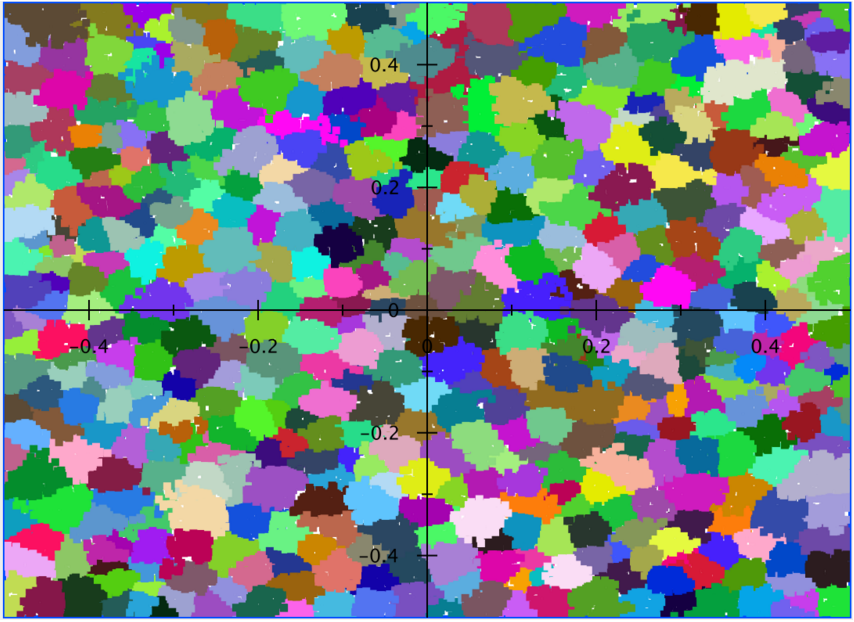
\includegraphics[width=0.6\linewidth]{onlinekm.png}
   \caption[BatchKM]{Online K-Means on a huge dataset with k=500.}
\end{figure}

\subsection{Adaptive Resonance Theory}
\subsubsection{The Algorithm}
Adaptive Resonance Theory (ART) \cite{ART} is set of neural network models that are used in supervised and unsupervised learning, pattern recognition and prediction. The ART algorithm for clustering follows an incremental approach where it starts the clustering by initializing the first data point as the cluster center and adds new clusters as new data is read. ART does not require the number of clusters to be specified, instead it requires a \textit{vigilance} value in order to create new clusters.

A vigilance parameter defines the degree of similarity between the data points in a cluster. In other words, the vigilance parameter controls which data would be suitable for a cluster. A larger vigilance value ensures that the cluster includes data points with lot of similar parameters resulting in a fine grained cluster. Whereas a lower vigilance value creates a cluster with more general, less detailed parameters.

In ART, initially the first input point is chosen as the centroid for the first cluster. When the Euclidean distance between the data point and its nearest centroid is less than the vigilance, then the update is calculated as in Online K-Means. However, if the distance is greater than the vigilance, then a new cluster is created with that point as a centroid.

For the data set $X = \left\{ {x^{t}}\right\}_{t=1}^N$, the following equations are performed for each update:
\begin{equation}
b_{i} = \parallel{m_{i}} - x^{t}\parallel  = \min_{l=1}^k \parallel  m_{l} - x^{t}∥
\end{equation}
 
\begin{equation}
\begin{cases}
m_{k+1}\leftarrow x^{t} & if b_{i}>\rho
\\\triangle{m_{i}}=\eta\left(x^{t} - m_{i}\right) & otherwise
\end{cases}
\end{equation}

where $m_{i}$ is the initial cluster center, $\rho$ is the vigilance value and $b_{i}$ is the  Euclidean distance between the point and its nearest centroid. 


\subsubsection{Implementation}
The ART algorithm has been implemented in Java. The \textit{Tools} class contains a set of multidimensional operations. The \textit{ART} class implements the \textit{update} function for each input data point, according to the equations 3.7 and 3.8. The variable \textit{row} is the user input vigilance value and \textit{point} is the next incoming data point. The method \textit{Tools.distance} returns the  Euclidean distance between the point and its nearest centroid.

\lstinputlisting[language=Java, basicstyle=\tiny, firstline=21,lastline=39]{ART.java}

If the distance between the point and the nearest centroid is less than the vigilance value, the method invokes the \textit{moveCentroid} function which adds the point to the cluster and updates the centroid. Otherwise the \textit{update} function creates a new centroid.

\lstinputlisting[language=Java, basicstyle=\tiny, firstline=40,lastline=45]{ART.java}

\begin{figure}[ht]
	\centering
	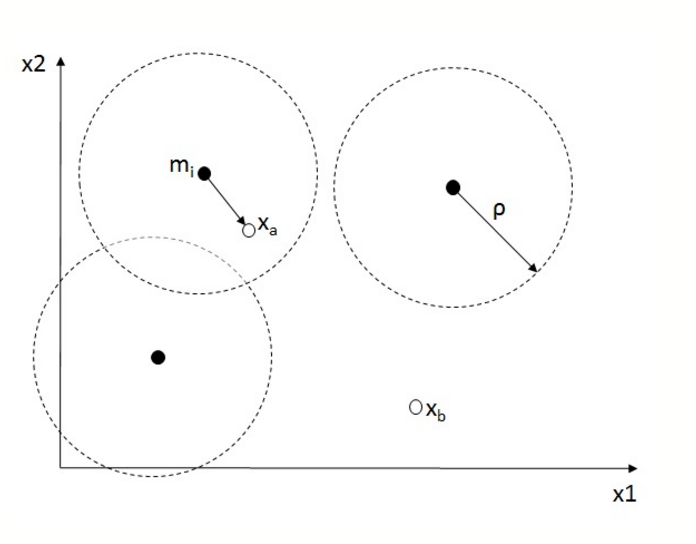
\includegraphics[width=0.8\linewidth]{artpic.png}
   \caption[ART]{ART algorithm}
    \footnotesize{Note: Adapted from \textit{Introduction to machine learning} by Ethem Alpaydn, p. 285, 2010. \cite{Clustering}}
 \end{figure}

\subsection{Silhouette}
\subsubsection{The Algorithm}
Silhouette is a method which allows one to measure how similar is a data point to all the other points in its cluster. This method is used to validate the consistency and strength of a cluster. The Silhouette Coefficient of a data point, $s(i)$ can be determined using the following formula:
\begin{equation}
s(i) = \frac{b(i) - a(i)}{max\left\{a(i), b(i)\right\}}
\end{equation}
which can also be expanded as,
\begin{equation}
s(i) = \begin{cases}
1-a(i)/b(i) & if a(i)<b(i)
\\0 & if a(i)=b(i)
\\b(i)/a(i) -1 & if a(i)>b(i)
\end{cases}
\end{equation}
where $a(i)$ is the average distance from the $i^{th}$ point to the other points in the same cluster and $b(i)$ is the minimum average distance from the $i^{th}$ point to points in a different cluster \cite{Rousseeuw}. The values $s(i)$ of a silhouette coefficient usually ranges between $-1$ and $1$. If $s(i)$ is close to 1, it means that the point is in the right cluster. If $s(i)$ is close to zero, then the point lies near the decision boundary of two neighboring clusters. Otherwise, if $s(i)$ has negative values, it means that the point is probably in the wrong cluster. The average silhouette values of all the points in the cluster is used to determine the quality of the clustering method used. Hence, the optimal number of clusters for an efficient clustering would be the number of clusters that gives the highest silhouette coefficient.

\subsubsection{Implementation}
The silhouette algorithm has been implemented in MATLAB using the function \textit{silhouette(X,clust,metric)} where $X$ is the matrix of data points, \textit{clust} is the cluster \textit{ids} of each data point and \textit{metric} is the inter-point distance function used. 

The variable \textit{data} is the path to the text file containing the data points while the variable \textit{kmeans} is the path to the text file containing their corresponding cluster numbers. The metric we used is the Euclidean distance between the points.

\lstinputlisting[language=Matlab, basicstyle=\tiny]{Silhouette.m}
The above program gives the mean Silhouette coefficient of the overall points in the cluster.

\clearpage
\section{Query Space Clustering}

The Online K-Means described at 3.1.3 provides an efficient approach to address huge data sets without accessing raw data. However, it is easy to notice that the input of Online K-Means (i.e., the output of queries) is randomly and uniformly chosen. This is obviously unreasonable. Thus, the challenge here is how to generate an appropriate input for Online K-Means. Before exploring the specific solution, it is necessary to give a definition for query and explain the generation of a query. 

\subsection{Original Query Generation}

A query Q has two parts: the input of the query, which is called \textit{query-point}, $\vec{x} $ and the \textit{radius} $ \theta $, where $\vec{x} $ is a multidimensional vector from the real dataset and $ \theta $ is the \textit{radius} with a constant value. 

\begin{equation}
	Q =[\vec{x},\theta] =[x_1,x_2,...,x_n,\theta] (n\ dimensions)
\end{equation}

For example, consider dealing with a dataset \textit{S} with two-dimensional points. The query-point is $\vec{x} = [x_1,x_2] $. In the Online K-Means mentioned before, the values of $ x_1\ and\ x_2 $ are chosen uniformly and randomly from \textit{S}. The next step is to scan whole data and gather a sub dataset, which includes all data points such that the Euclidean distance between a point, for example in two dimensions, $ Z = [z_1,z_2]$ and the query-point $ [x_1,x_2] $ is less than  $ \theta $. i.e., $$ \sqrt{(x_1-z_1)^2 + (x_2-z_2)^2} < \theta $$ Subsequently, record the average of all points that satisfy the criterion: less than  $ \theta $, and notate this as the output of a query. $$ average = \frac{\sum_{i=1}^{n} Z_i}{n} $$ Finally, if there are \textit{M} queries, repeat this process of query generation for \textit{M} times and save all the output as the input for Online K-Means. 

\subsubsection{Implementation}
The original query generation was implemented in Java. The methods are shown below:

\lstinputlisting[language=Java, basicstyle=\tiny, firstline=49,lastline=60]{OriginalTools.java}

This function is used to generate a set of queries randomly with two parameters: \textit{int queryLimit} (i.e., M queries) and \textit{int noOfAxis} (i.e., the dimensions of points). \textit{r.nextFloat()} returns the next uniformly distributed float value between 0.0 and 1.0; then we subtract 0.5 simply because the range of the dataset, in our case, is between -0.5 to 0.5.

\lstinputlisting[language=Java, basicstyle=\tiny, firstline=25,lastline=30]{OriginalTools.java}
The \textit{for} loop scans the whole data space \textit{dataSet} and compares each Data point \textit{d} with a query point(\textit{query}) to find points that the have distance less than $ \theta $ between each other and finally save the points in the List \textit{dataInTheta}. 
\lstinputlisting[language=Java, basicstyle=\tiny, firstline=15,lastline=21]{OriginalTools.java}
This function \textit{Tools.distance()} can calculate the two dimensional Euclidean distance between two points \textit{Data p1} and \textit{Data p2}. \textit{xdist} and \textit{ydist} represent the distance for each dimension.
\lstinputlisting[language=Java, basicstyle=\tiny, firstline=33,lastline=47]{OriginalTools.java}
The idea here is to use a loop to count the sum of the points within the List \textit{dataInTheta} for all dimensions respectively and then, compute and store the mean value for each dimension in an float array. Finally, this array is packaged as an average point structure: \textit{Data}. 

However, the idea of original query generation has two limitations. Firstly, as mentioned above, users are less likely to issue queries from whole dataset uniformly and randomly. Another problem is that this method needs to scan the entire dataset once for each query. It may cause a heavy load and high cost for computers especially when addressing a large-scale dataset. Query Space Quantization (i.e., Query Space Clustering) is proposed to solve these problems. 

\subsection{Pre-define Data Subspaces by Interest Points}
To begin with, it is necessary to pre-define some data subspaces in order to simulate the user's areas of interest. Assume that there are 10 subspaces in a 2-dimensional dataset. That is, the user normally issues queries from these ten data subspaces. More specifically, fix a data space, say space L, L = $ \{l_1,l_2, ..., l_{10}\} $. Each subspace in L is modeled through a Gaussian distribution of 2 dimensions, i.e., a mean value $ \mu_1 $ for dimension 1 and a mean value $ \mu_2 $  for dimension 2 are needed, $ l_i= (\mu_1,\mu_2) $. Furthermore, for simplicity, assume that the standard deviation  $ \sigma_1 $  and $ \sigma_2 $ for both dimensions are the same and fixed, e.g., $ \sigma = \sigma_1 $ = $ \sigma_2 $ = 0.01. 

\begin{figure}
	\subfigure[Input of L]{
	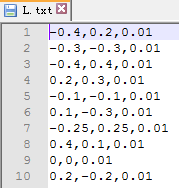
\includegraphics[width=.2\textwidth]{Ltxt.png}
	}
	\subfigure[Visualization of query points in L]{
	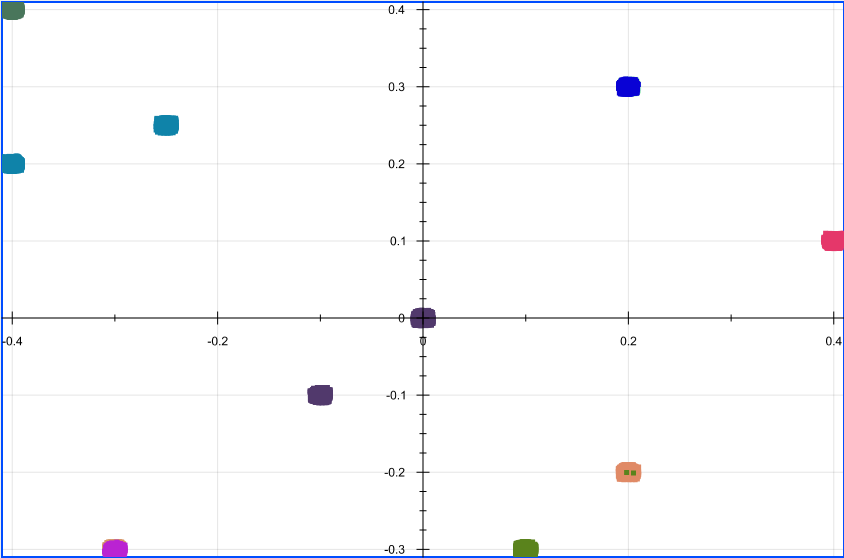
\includegraphics[width=.38\textwidth]{L.png}
	}
	\subfigure[Zoom in to $ l_9 $=(0,0)]{
	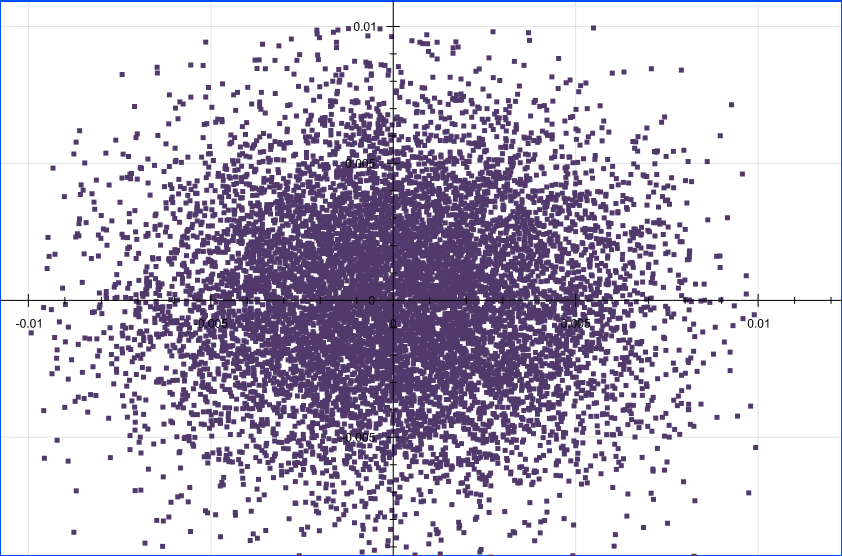
\includegraphics[width=.38\textwidth]{Gaussian.png}
	}

Figure (a) is a screenshot for the input file L, which pre-defines ten centers for ten subspaces. The format follows $ (\mu_1,\mu_2,\sigma) $. Figure (b) and (c) show that the query points generated by Gaussian distribution can form a disc around the input from figure (a). The implementation details will be introduced in the next section.
\end{figure}

\subsection{Select a Subspace and Generate a Query}
Initially, assume that there is a need to generate \textit{N = 10000} queries from L = 10 subspaces. That is, a subspace in L is firstly chosen from 1 to 10, each one with equal probability, i.e., Random($ l_1,...,l_{i},...,l_{10} $), \textit{i} = (1...10). Intuitively, 10000/10 = 1000 queries will be generated from each subspace. Next, in order to generate a query Q = $ [x_1,x_2,\theta] $ from the \textit{i-th} subspace, it is necessary to set the center of query-points, $ l_i=(\mu_1,\mu_2) $ , and the $ \theta $ is fixed, e.g., $ \theta=0.1 $. The  $ x_1 $ is generated by the Gaussian with mean value $ \mu_1 $ and variance $ \sigma^2 $ ($ Reminder: \sigma = \sigma_1 $ = $ \sigma_2 $ = 0.01). The same holds true for $ x_2 $. That is,  $ x_1 $ = Random.Gaussian($ \mu_1 $,$ \sigma^2 $) and  $ x_2 $ = Random.Gaussian($ \mu_2 $,$ \sigma^2 $). Hence, the query Q = $ [x_1,x_2,\theta] $ with the center of query-points $ l_i=(\mu_1,\mu_2) $ is located within the \textit{i-th} subspace, i.e., in a disc of center $ (\mu_1,\mu_2) $.

\subsubsection{Implementation}
The generation of query-points, which follow Gaussian distribution, was implemented in Java as well. The function is presented below:
\lstinputlisting[language=Java, basicstyle=\tiny, firstline=102,lastline=117]{Tools.java}
\lstinputlisting[language=Java, basicstyle=\tiny, firstline=10,lastline=14]{Tools.java}
There are two parameters: \textit{float[] point} represents the center $ (\mu_1,\mu_2) $, \textit{float width} means the standard deviation  $ \sigma $. \textit{r.nextGaussian()} returns the next Gaussian distributed double value with mean 0.0 and standard deviation 1.0. Multiplying it by (\textit{width/3}) enables that about 99.7\% of a population will be within the range (-$ \sigma $, +$ \sigma $). Finally, we move this point towards the center by adding the mean value $ \mu_1 $ and $ \mu_2 $ respectively. 



\subsection{Online Quantization}
Finally, the concept here is to address the problem of time-consuming and high cost for executing a query over large-scale dataset by avoiding storing all the queries and scanning all dataset. In the reality where users issuing queries, it is essential to quantize them \textit{online}. That is to incrementally generate queries and then injecting each one to the online K-means algorithm, for quantizing the query vectors. Obviously, if K equals the number of subspaces in L, then after a lot of queries, it can be seen that all the K-means vectors will be the vectors with dimensions ($ \mu_1[i] $, ..., $ \mu_n[i] $) since, naturally, the K-means algorithm learn the query distribution, which in this case in a 10-modal Gaussian distribution, i.e., 10 Gaussian bells.

\subsubsection{Implementation}

\lstinputlisting[language=Java, basicstyle=\tiny, firstline=123,lastline=129]{QueryClustering.java}
\textit{int queryLimit} in this part of \textit{for} loop is the number that represents M queries. The function \textit{printQueryCompletion()} is just to report the process to console, so ignore it. \textit{Tools.generateQuery()} can produce a query vector as decribed above. \textit{queriesOnline.update()} calls the online K-means and returns the closest centroid id. The centroid can also be acquired by \textit{queriesOnline.getCentroids()}. Thus, it means, for each query, inject it to online K-Means and then repeat M times. 


\clearpage
\section{Prediction}
Within the prediction sections 3.1 and 3.2 with their described techniques are join up with each other but only under consideration of two dimensional data. The intent outcome of the prediction is to find the average data point of a query without scan through the behind dataset. 

In order to achieve this, a training set is needed to learn the machine algorithm and finally test with another dataset how good this learning was. The goodness of this machine learning algorithm, the exact evaluation, will be explained in chapter 4. In this section the implementation of creating the training and test set, learning the algorithm and predict the outcome from a query input will be described in the following subsections. Each subsection represents a standalone application which can be run through the generated batch file with modifying the depending input variables. 

\subsection{Mapping query and output data}

The fundamental for a successful prediction is to create a training set that is mapping the query that was generated through the actual output, the average data point.

A query is defined in equation 3.7 with a point \textit{x} for each dimension and the radius theta, a constant in our work.  
\begin{equation}
q=[x_1,x_2,\theta] =[\vec{x},\theta]
\end{equation}
For each query an output, containing the average data point of all data points from the real dataset inside the defined radius theta, will be generated. Therefore the output of a query is defined as:
\begin{equation}
\bar{x}=[\bar{x_1},\bar{x_2}]=\frac{1}{n}\sum \vec{x_i}:\parallel \vec{x}-\vec{x_i}\parallel \leq \theta
\end{equation}
Figure \ref{fig:Query} visualizes this technique by showing a two dimensional dataset, representing a query with a blue point and a dashed line for the radius theta, the actual dataset points with a black point and the average data point with a red one.
 \begin{figure}[ht]
	\centering
	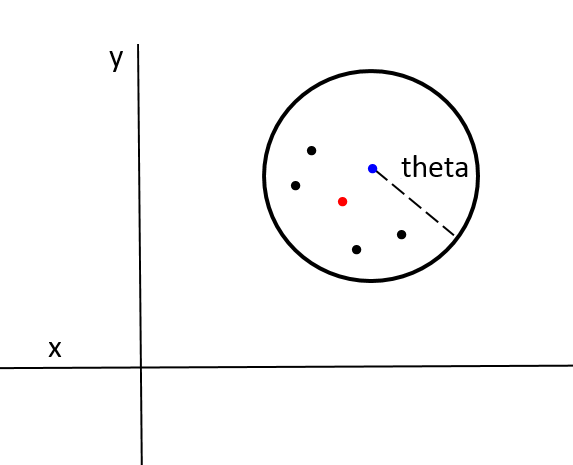
\includegraphics[width=0.5\linewidth]{Query.PNG}
	\caption[Query]{Query and average data point creation}
	\label{fig:Query}
\end{figure}

The exact approach and implementation will be found in section 3.2.1.. With our definition of query and the related output for each query we can define our training set as:
\begin{equation}
Trainingsset=[q,\bar{x}]
\end{equation}

\subsubsection{Implementation}

The application for mapping a query and the average data point is implemented in Java; an extract of the java class QueryGE is presented below:

\lstinputlisting[language=Java, basicstyle=\tiny, firstline=42,lastline=58]{QueryGE.java}

Inside the \textit{for} loop a random query will be generated with the method \textit{generateQuery()} inside the ranges of the defined subspace explained in section 3.X; if no subspace is defined the query will will be generated over the whole dataset. After a query is generated the average data point for this query will we located through the method \textit{generateAverageDataFromQuery()}. Both query and average data point are stored in a float array. The final coordinates of the query and the average point will than be written into a semicolon separated file using \textit{BufferedWriter}.

The whole application \textit{TrainingSetAppliction} can be run by giving a dataset, theta, a number of queries and a file with subspaces the user is interested in.
After training the machine learning algorithm a test set is needed with the same structure of the training set; therefore this application can be used also for creating the test set. 


\subsection{Learning algorithm}

In order to process the learning from the previously generated training set we can use the online k-means algorithm. This concept was explained in section 3.1.3.
A short summary of the key facts: the online k-means sets the first k points as cluster centroids and moves the nearest centroid for the next point in its direction with a fixed alpha. The following paragraph will explain how we connected the online k-means approach with our training set and how we created our set for the prediction.

To find the centroid of all queries we give them one by one to the online kmeans algorithm. At the same time another instant of the online k-means gets the related average point. This is implemented in our java class \textit{LearningApplication} in row 64-65, see following code extract:

\lstinputlisting[language=Java, basicstyle=\tiny, firstline=64,lastline=65]{LearningApplication.java}

The important thing is that the connection between the cluster of a query and the average point is still established. Wherefore we store the cluster id of our average data on the same position of the query cluster id. This can be seen in this code extract:
\lstinputlisting[language=Java, basicstyle=\tiny, firstline=66,lastline=66]{LearningApplication.java}

Thanks to this, after running the online k-means through the whole training set, we have a list of cluster id of our average data on the position of the query cluster id. As a result we can write the centroid of our queries, defined in equation 3.10, with the related centroid of the average data, defined in equation 3.11, in a file by using \textit{BufferedWriter}. See posterior code detail:
\lstinputlisting[language=Java, basicstyle=\tiny, firstline=70,lastline=82]{LearningApplication.java}

Therefore our prediction set will be containing the centroid of our queries w[j] and the correspondent centroid of the average data u[j], see the following notations for definition.
\begin{equation}
w[j]= online\,k-means\,centroids\,for\,q
\end{equation}
\begin{equation}
u[j]= online\,k-means\,centroids\,for\,\bar{x}
\end{equation}
\begin{equation}
Prediction\,set=[w[j],u[j]]
\end{equation}

\subsection{Prediction algorithm}

In the last application our previous generated prediction and a new test set will be used to predict for each query inside the test set an average data point without scanning through the dataset.

To predict the average point we try to find for each query the alike query-centroid. This can be done by using the nearest neighbour algorithm. It is calculation the euclidean distance between a point and a list of points and gives you for this point the nearest. For more details and the exact implementation go to section 3.1.1. We need to search for the nearest query centroid for this query in order to find the correspondent average data centroid and declare it as our predicted \textit{xbar}.  

This logic is implemented with the java class \textit{PredictionApplication}:
\lstinputlisting[language=Java, basicstyle=\tiny, firstline=66,lastline=69]{PredictionApplication.java}

Within this extract the method \textit{classify()}, which is explained in section 3.1 with more detail, is invoked. This method takes the list of centroids and the new query of the test set as input and returns the nearest centroid of queries for the input query. Afterwards the centroid of the average data is easily found and marked as our predicted \textit{xbar}.

To evaluate the goodness of our predicted \textit{xbar}, we can define an error value for each query. This error value is defined in 3.13 as the euclidean distance between the predicted \textit{xbar}, our centroid, and the actual \textit{xbar}.

\begin{equation}
	\epsilon_i = \parallel \bar{x} - u[j] \parallel 
\end{equation}

\lstinputlisting[language=Java, basicstyle=\tiny, firstline=71,lastline=74]{PredictionApplication.java}

For a summary evaluation it is possible to calculate the mean error over the test set by summing each error and divide it through the number of queries in the test set. The mean error is defined in equation 3.14.

\begin{equation}
Mean\,Error= \frac{\sum\epsilon_i}{i}
\end{equation}

\lstinputlisting[language=Java, basicstyle=\tiny, firstline=79,lastline=79]{PredictionApplication.java}

Further evaluation can be done by reading the result file that will be produced through the prediction. This file contains, for each query, the predicted average data point and, the actual data point and the error value. At the end of this file the mean error is displayed. 
%==============================================================================
\chapter{Evaluation}
For the algorithm k-means (batch and online), ART and query space we used a dataset about gas sensor data from the machine learning repository of UIC\cite{dataArchive}. The Gas data we used contains 5 sensors (columns) and is limited to the first 500,000 rows because of memory issues during the silhouette evaluation. For the prediction part only 2 sensors were taken so that we could better visualize the data and results we were achieving.

\section{Silhouette}
Silhouette is an algorithm that validates the consistency and strength of a cluster. This algorithm was described in detail in Section 3.1.5.
A mean Silhouette value between 0 to 1 means a good cluster. If the value is 1 it means a perfect cluster. For values between 0 and -1 the points are mostly not in the nearest or best cluster.

\subsection{K-means}
Batch and Online K-Means were tested as well with different values of $k$ ($50,150,400$) and $theta$ ($0.05,0.2$) for the queries. For K-Means functions the number of radius queries is $100.000$.

If we compare online and offline k-means over real data (see table below) we can see that online k-means is producing a better silhouette value than the offline k-means in case of 150 cluster. Therefore it can assume that the online k-means is as good as the offline k-means, sometimes even better.

\begin{tabular}{|c|c|c|c|}
	\hline  & K=50 & K=150 & K=400 \\ 
	\hline Batch K-means &  & 0.3584 & out of memory \\ 
	\hline Online K-Means &  & 0.4713 &  \\ 
	\hline 
\end{tabular} 

The silhouette value over queries for $theta$ $0.05$ and $0.2$ using online and batch k-means is displayed in the following tables. For $theta$ $0.05$ no silhouette values could be created. This is due to the fact that with $theta$ $0.05$ the search space next to the query is very small, thus, many queries don't return any results. 

\begin{tabular}{|c|c|c|c|}
	\hline Theta=0.2 and M=10k & K=50 & K=150 & K=400 \\ 
	\hline Batch K-Means & 0.2569 & -0.0815  & -0.1345  \\ 
	\hline Online K-Means & 0.339 & 0.2894 & NaN \\ 
	\hline 
\end{tabular}

\begin{tabular}{|c|c|c|c|}
	\hline Theta=0.2 and M=100k & K=50 & K=150 & K=400 \\ 
	\hline Batch K-Means & 0.4163 & 0.3025  & 0.2492  \\ 
	\hline Online K-Means & 0.3778 & 0.3337 & 0.2579 \\ 
	\hline 
\end{tabular} 

\begin{tabular}{|c|c|c|c|}
	\hline Theta=0.2 and M=200k & K=50 & K=150 & K=400 \\ 
	\hline Batch K-Means & 0.1899 & 0.0767  & -0.0252  \\ 
	\hline Online K-Means & 0.3719 & 0.3402 & 0.2808 \\ 
	\hline 
\end{tabular}

From the above tables one can see that the online k-means seems to be performing more consistently then the batch k-means. From the tables we can conclude that as K increased the silhouette values decreased as well. This is probably due to the case that K was getting too high for the number of Data Points. The silhouette values increased as the number of queries increased, since the more queries that are ran the greater the number of data points to cluster. The only exception occurred for the batch kmeans at 200,000 queries where the results were expected to improve but instead had a very low value. On average it also seemed that the online provided better silhouette values.

Another important thing to note is that the although the Real Data gave better results, the average data which has much less data points still gave very similar silhouettes. This helps us conclude that we don't need to have the actual data but can instead work with the average data.

\subsection{ART}
For a better understanding of the impact of vigilance and theta values in ART, we tested the algorithm with different values for both variables, evaluating the average clustering results with silhouette. As we already mentioned before, silhouette algorithm computes the average result for all the cluster evaluations. It is possible to notice that the performance is proportional to theta; however, for greater vigilance values the difference in performance as theta varies becomes more negligible.
The number of radius queries generated and executed over the original data space in order to test ART is $200.000$. In figure 4.1 the 3D plot with the relation between vigilance, theta and the mean silhouette value is shown. The following table shows the exact values of silhouette for each theta (row) and vigilance (column).

\begin{figure}[ht]
	\centering
	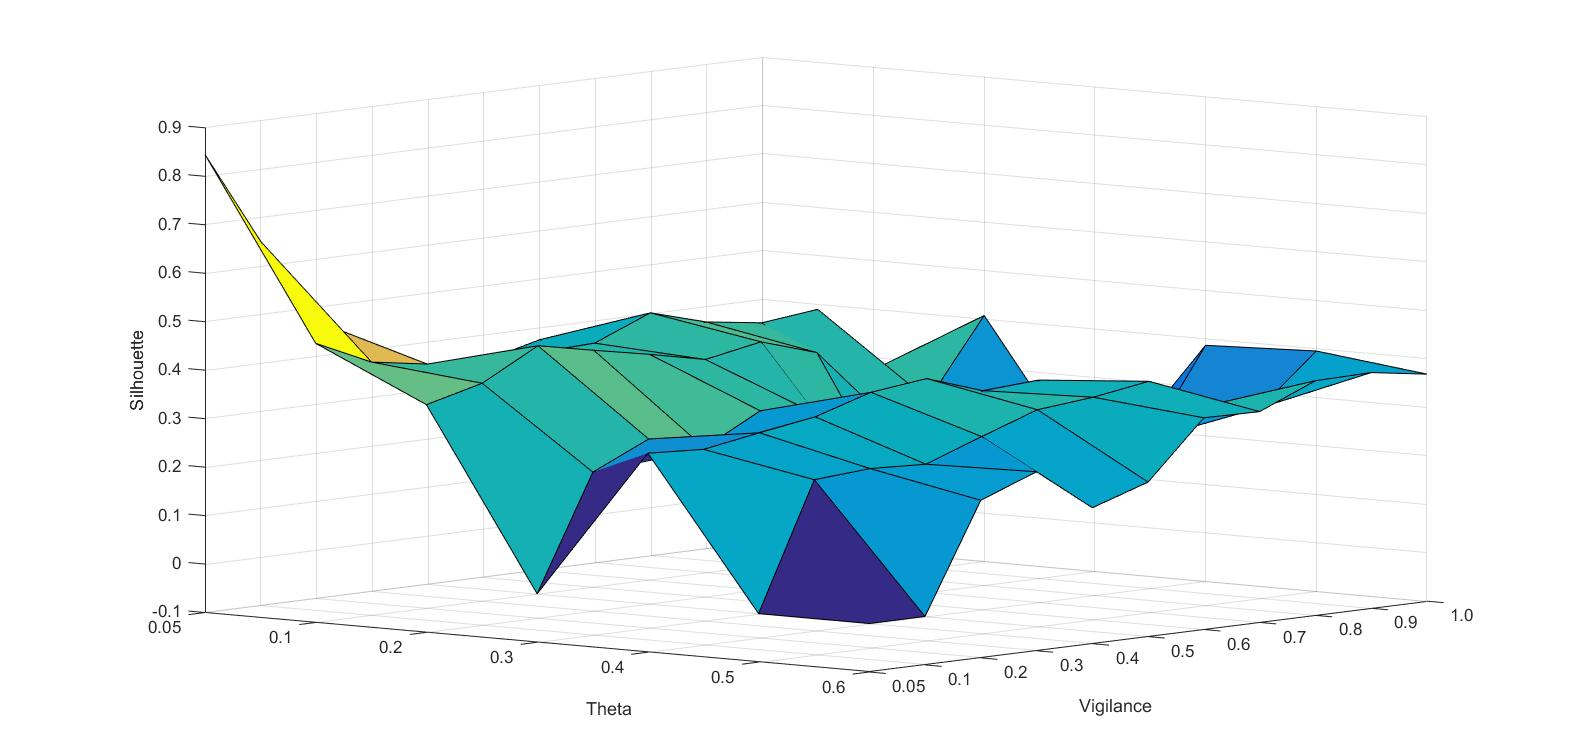
\includegraphics[width=1.1\linewidth]{Evaluation_ART.jpg}
   \caption[ARTevaluation]{The impact of Theta and vigilance in ART}
\end{figure}

\begin{tabular}{|c|c|c|c|c|c|c|c|c|c|c|c|}
		\hline    & 0.05   & 0.1    & 0.2    & 0.3    & 0.4    & 0.5    & 0.6    & 0.7     & 0.8    & 0.9    & 1.0   \\ 
		\hline 	0.05 & 0.8448 & 0.6508 & 0.4719 & 0.3514 & 0.3125 & 0.3458 & 0.3752 & 0.3117  & 0.3271 & 0.3083 & 0.3083 \\
		\hline 	0.1  & 0.4757 & 0.4226 & 0.4038 & 0.3974 & 0.3981 & 0.4032 & 0.4511 & 0.4177  & 0.4013 & 0.4145 & 0.2752 \\
		\hline 	0.2  & 0.3697 & 0.3993 & 0.4621 & 0.4381 & 0.4152 & 0.3899 & 0.4117 & 0.3749  & 0.2501 & 0.2481 & 0.4076 \\
		\hline 0.3  & NaN      & 0.2365 & 0.2902 & 0.2573 & 0.3191 & 0.2981 & 0.1307 & -0.0128 & 0.1476 & 0.1539 & 0.0862 \\
		\hline 	0.4  & 0.3105 & 0.3038 & 0.3234 & 0.3417 & 0.3777 & 0.3914 & 0.3519 & 0.3591  & 0.2602 & 0.2086 & 0.387  \\
		\hline 	0.5  & NaN      & 0.2617 & 0.27   & 0.2644 & 0.3068 & 0.3476 & 0.3588 & 0.377   & 0.311  & 0.2933 & 0.3957 \\
		\hline 	0.6  & NaN      & NaN      & 0.2251 & 0.2693 & 0.1804 & 0.2188 & 0.3368 & 0.3349  & 0.3841 & 0.3862 & 0.3684 \\
		\hline
\end{tabular}


\section{Query Space}

For evaluating the query space we do not cluster the query output instead we clustered the actual query. To evaluate this we developed a visualization tool to help us see the actual results.

\begin{figure} [h]
	\subfigure[Real data]{
	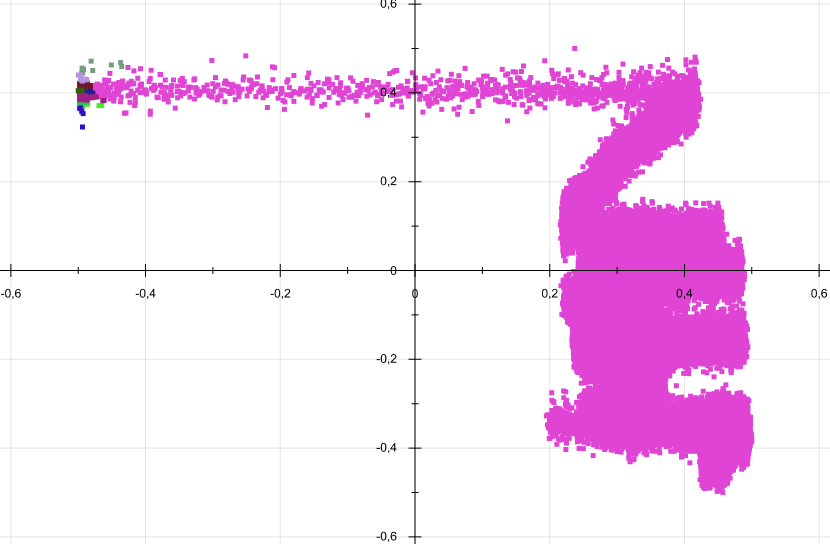
\includegraphics[width=.5\textwidth]{real.PNG}
	}
	\subfigure[Real data subspace output]{
	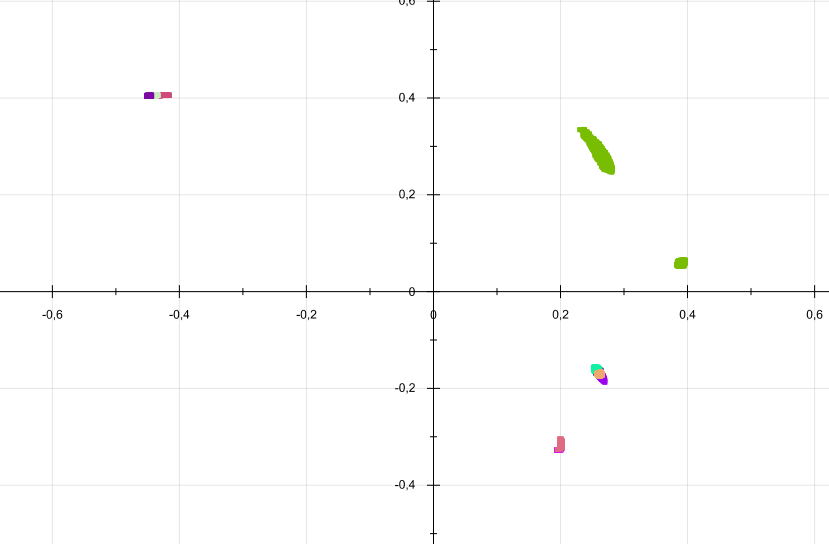
\includegraphics[width=.5\textwidth]{query_real.PNG}
	}
\end{figure}
 
To evaluate this the similarity between queries was checked by using kmeans and plotted over the space to compare the positions of the queries with their center points. This is shown in the following table.

\begin{figure}[h!]
\centering
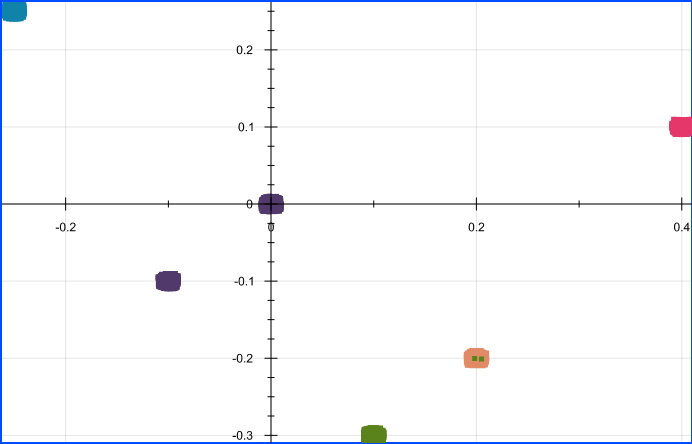
\includegraphics[width=.5\textwidth]{inputOfQuery.png}
\caption{Query points distribution}
\label{qpd}
\end{figure}

\begin{tabular}{|c|c|c|c|c|c|c|}
	\hline   & No.1 & No.2 & No.3  \\ 
	\hline Mean value of query points & (-0.25,0.25) & (-0.1,-0.1) & (0,0)  \\ 
	\hline Centroid of query cluster & (-0.1522,0.2484) & (-0.0912,-0.1108) & (-0.0628,-0.0023) \\ 
	\hline Euclidean Distance & 0.097813 & 0.013931 & 0.062842 \\
	\hline   & No.4 & No.5 & No.6 \\ 
	\hline Mean value of query points &  (0.1,-0.3) & (0.2,-0.2) & (0.4,0.1) \\ 
	\hline Centroid of query cluster & (0.117,-0.3465) & (0.2653,-0.2567) & (0.4115, 0.0255) \\ 
	\hline Euclidean Distance & 0.04951 & 0.086481 & 0.075382 \\	
	\hline
\end{tabular}

The image above shows the plotted queries and the different colors show the individual clusters. The center of these clusters should be the same as the specified L - which is the user interest points. As one can see the able gives the euclidean distance between the L and cluster centroids which is very small.

\section{Error}
To properly evaluate our system we began by generating a training and evaluation set. As previously explained the training set is used to learn and then the evaluation set is used to predict results. Since this is an evaluation set the predicted results are compared with their actual results and the difference calculated. The difference is the error. To evaluate the prediction this process was repeated 5 times using a training set of size 50,000 and evaluation size of 20,000. The mean errors ranged between 0.057 and 0.05 which means around 5\% error since the data space range was between -0.5 and 0.5.

%==============================================================================
\chapter{Conclusion}
We have studied a novel solution to the problem of predictive analysis over distributed data. This query driven solution is able to abstract query similarity and cluster the underlying data. The query clusters are associated with their related underlying data. The results of new queries are predicted by using the most similar query cluster. We evaluated this solution by using an evaluation data set to confirm that the predicted results are similar to the actual results. The significance of this study lies on the fact that it can predict results with restricted access to the dataset. This is due to the how the online learning mechanism is implemented, the prediction and learning steps are independent to the dataset, thus offering a scale-out and decentralized solution. 

\section{Future work}

Each subspace is chosen from L with an equal probability which is a rare situation in reality. Some probability theories and predictive methods could be implemented, such as Bayesian inference. Currently Gaussian distribution is used which is very common but other models could also be considered such as linear regression. Combining together some inference theories, can result in a more accurate approximation.

To generate the training set queries are executed over the real data and this process is currently very optimized. The distance between each query and data point is checked but this is extremely slow as it scales linearly with the size of the data. A data structure to minimize the number of data points to be checked can be implemented to reduce the time to generate the training set.

%==============================================================================
\section{Contributions}
Kurt Portelli worked on the 
%introduction, related work, conclusion, 
query generation code 
%and helped out with various other parts of the system
. Ruben Giaquinta worked on the batch K-means code and %Clustering parts of the report. 
Natascha Harth took care of the 
%prediction chapter of the report and 
silhouette script. Xu Zhang was responsible for the 
%Query Space Clustering part of the report and 
Data normalization code. Monica Ghandi worked on the Online K-means. Everyone was involved and helped in the implementation of ART and the prediction. %of the system and evaluation section.
%==============================================================================
\bibliographystyle{plain}
\bibliography{example.bib}

\end{document}

